\clearpage
\thispagestyle{empty}
%\pagenumbering{gobble}
\chapter*{Apêndices}
\addcontentsline{toc}{chapter}{Apêndices}
\pagestyle{plain}
\newpage
\newpage
\section{Apêndice A.1.}

Cópia do artigo \enquote{Mapping bias overestimates reference allele frequencies at the HLA genes in the 1000 Genomes Project phase I data}: \emph{G3: Genes|Genomes|Genetics} (2015), 5(3): 931-941.

Neste artigo, eu contribuí com o planejamento das análises e
na compreensão da organização dos dados do Projeto 1000 Genomas. Além disso, realizei alguns dos testes estatísticos e propus a utilização de medidas de desvio de frequência. Finalmente, contribuí com comentários acerca da redação do texto.


%%%%%%%%%%%%%%%%%%%%%%%%%%%%%%%%
%%%%%%%%%%%%%%%%%%%%%%%%%%%%%%%%
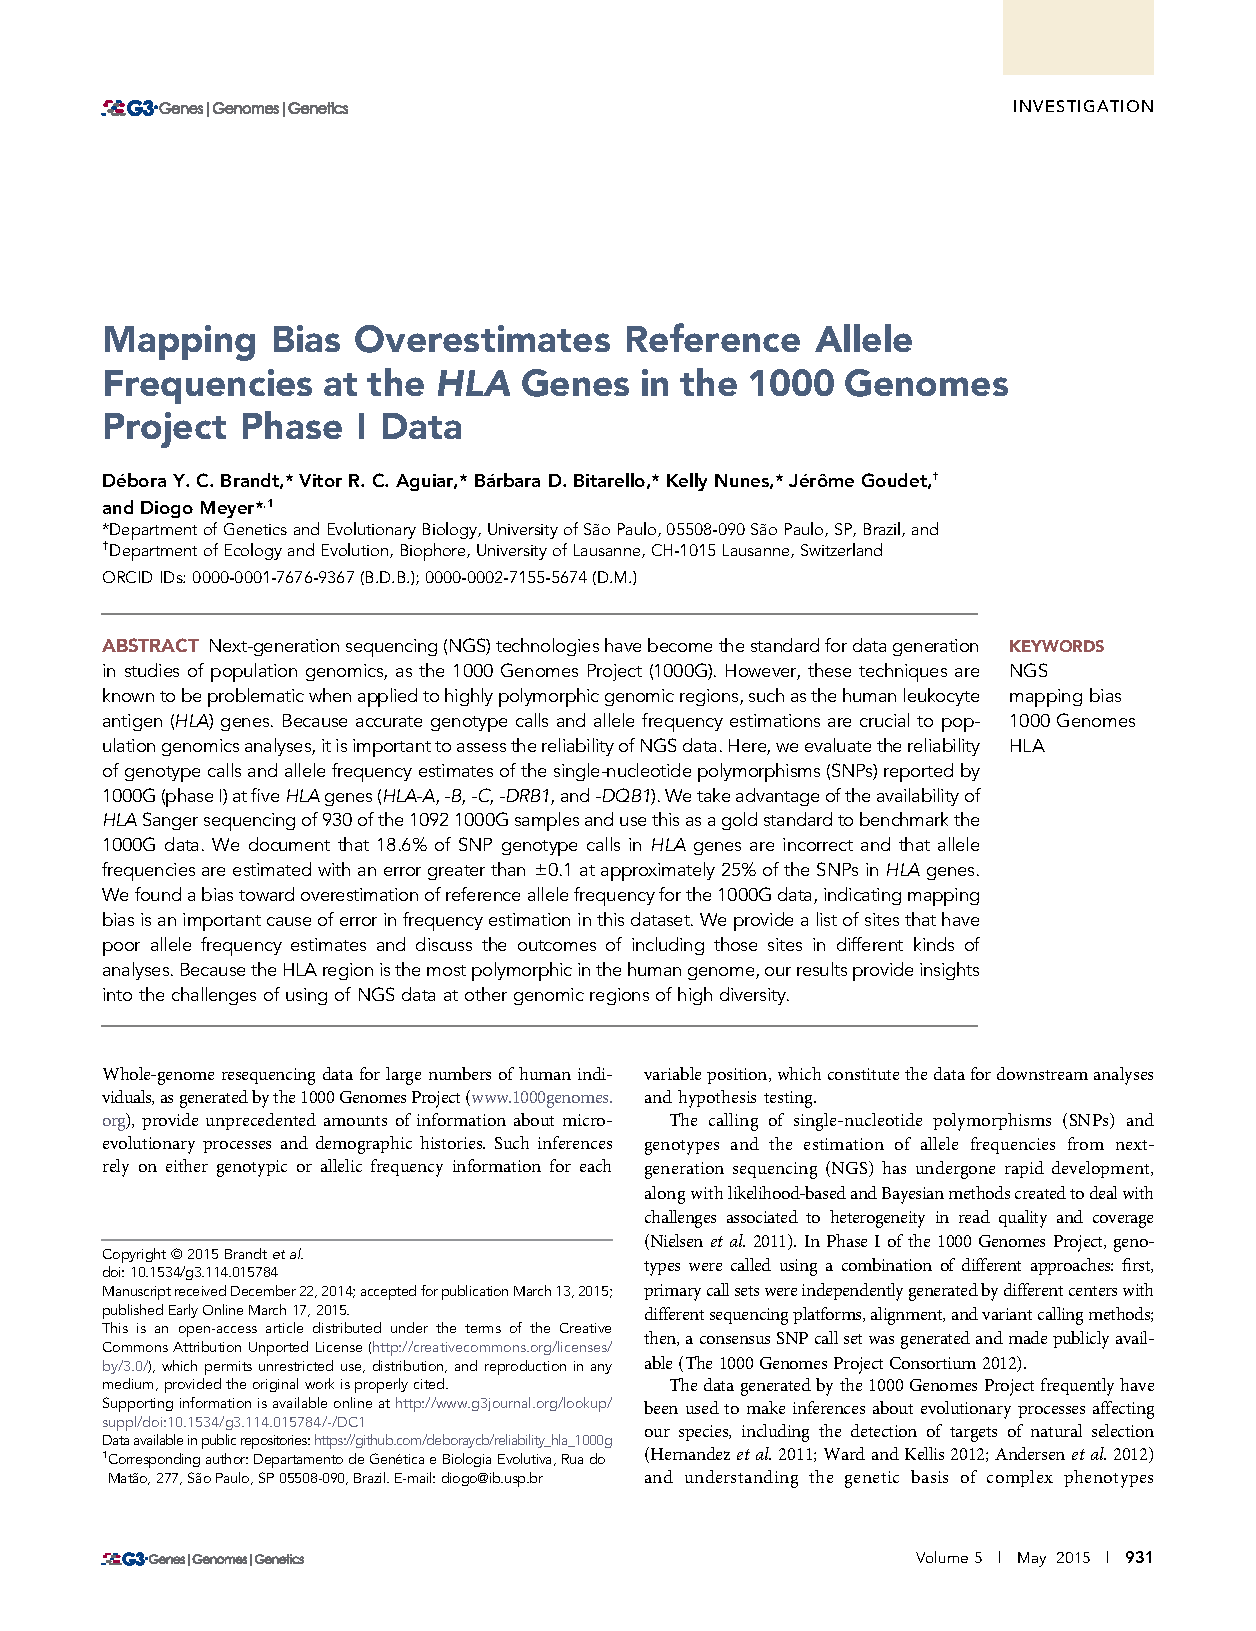
\includepdf[
            pages=-,
            width=189mm,
            height=253mm,
            offset=15pt 0pt,
            pagecommand={\pagestyle{plain}}
            ]
            {Appendix/small_G3brandt.pdf}
%%%%%%%%%%%%%%%%%%%%%%%%%%%%%%%%

%%%%%%%%%%%%%%%%%%%%%%%%%%%%%%%%
%%%%%%%%%%%%%%%%%%%%%%%%%%%%%%%%
\section{Apêndice A.2.}

Cópia do artigo \enquote{HLA supertype variation across populations: new insights into the role of natural selection in the evolution of HLA-A and HLA-B polymorphisms}: \emph{Immunogenetics} (2015), 67(11):651-663.

Neste trabalho, contribuí com \emph{scripts} em Perl para a realização das permutações descritas no artigo. Além disso, este trabalho tem fortes pontos em comum com o manuscrito apresentado no Apêndice A.4: em ambos, investigamos as unidades de seleção nos genes HLA, ainda que com abordagens bastante distintas. Aqui, trabalhamos com os genes \emph{HLA-A} e \emph{HLA-B} em um contexto populacional, e investigamos o papel dos supertipos como unidades de seleção, ao passo que no outro (A.4) usamos abordagens filogenético-comparativas para investigar o papel das linhagens alélicas de HLA como unidades de seleção nos genes HLA de classe I. 
%melhorar
%%%%%%%%%%%%%%%%%%%%%%%%%%%%%%%%
%%%%%%%%%%%%%%%%%%%%%%%%%%%%%%%%
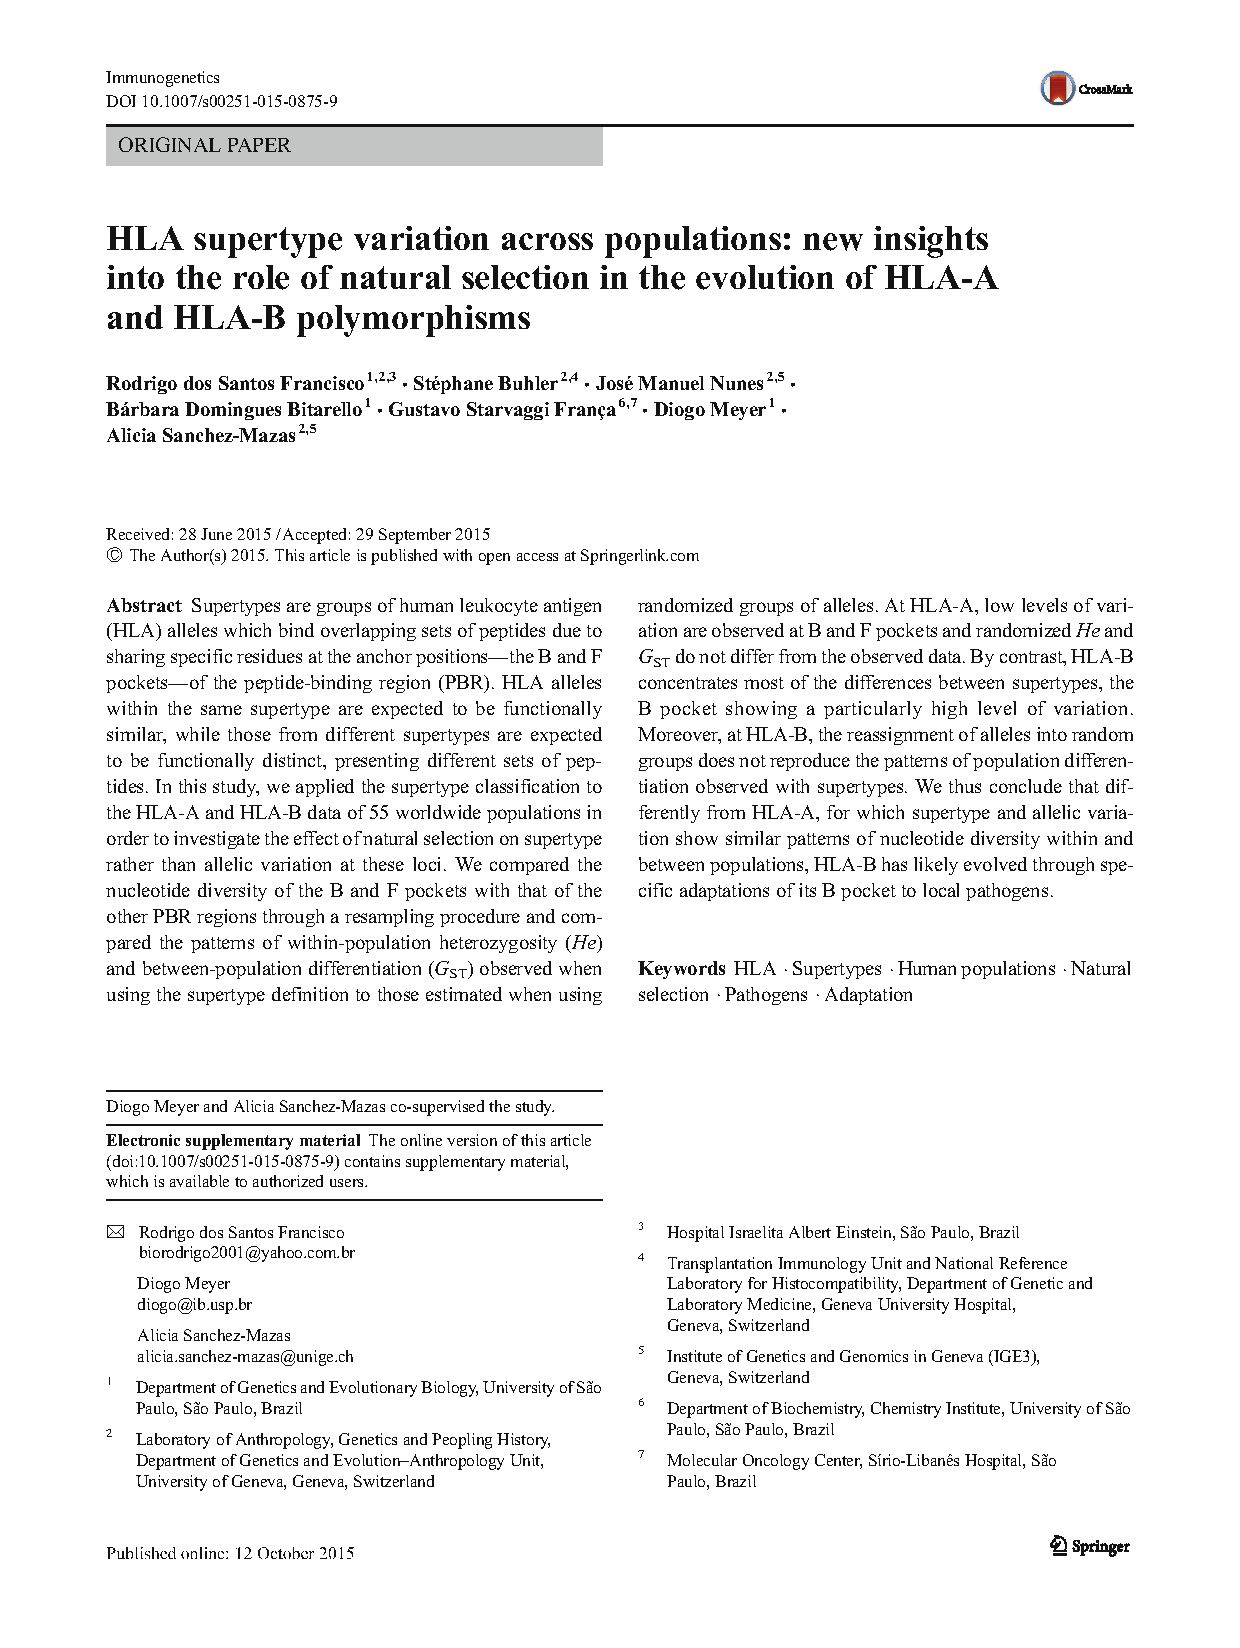
\includepdf[
			pages=-,
            width=189mm,
            height=260mm,
            offset=15pt 0pt,
            pagecommand={\pagestyle{plain}}
            ]
            {Appendix/art_3A10_1007_2Fs00251-015-0875-9.pdf}
%%%%%%%%%%%%%%%%%%%%%%%%%%%%%%%%%%%%%%%%%%%%%%%
%%%%%%%%%%%%%%%%%%%%%%%%%%%%%%%%%%%%%%%%%%%%%%%
\section{Apêndice A.3.}

Cópia do artigo \enquote{Kiwi genome provides insights into evolution of a nocturnal lifestyle}: \emph{Genome Biology} (2015), 16(1): 1-15.

Neste trabalho, eu realizei os testes de seleção baseados em $dN/dS$ usando o pacote PAML -- e/ou supervisionei sua execução e interpretação --  e fui responsável pela discussão dos resultados referentes a estas análises no artigo. Também fiz parte das análises referentes às regiões ultra-conservadas (\emph{Ultra-conserved non-coding elements}) que apresentam mais variação do que o esperado em kiwi, indicando possíveis vias de desenvolvimento alteradas nessa espécie. Finalmente, contribuí com correções do manuscrito e com discussões relacionadas aos aspectos evolutivos do trabalho.

%%%%%%%%%%%%%%%%%%%%%%%%%%%%%%%%
%%%%%%%%%%%%%%%%%%%%%%%%%%%%%%%%
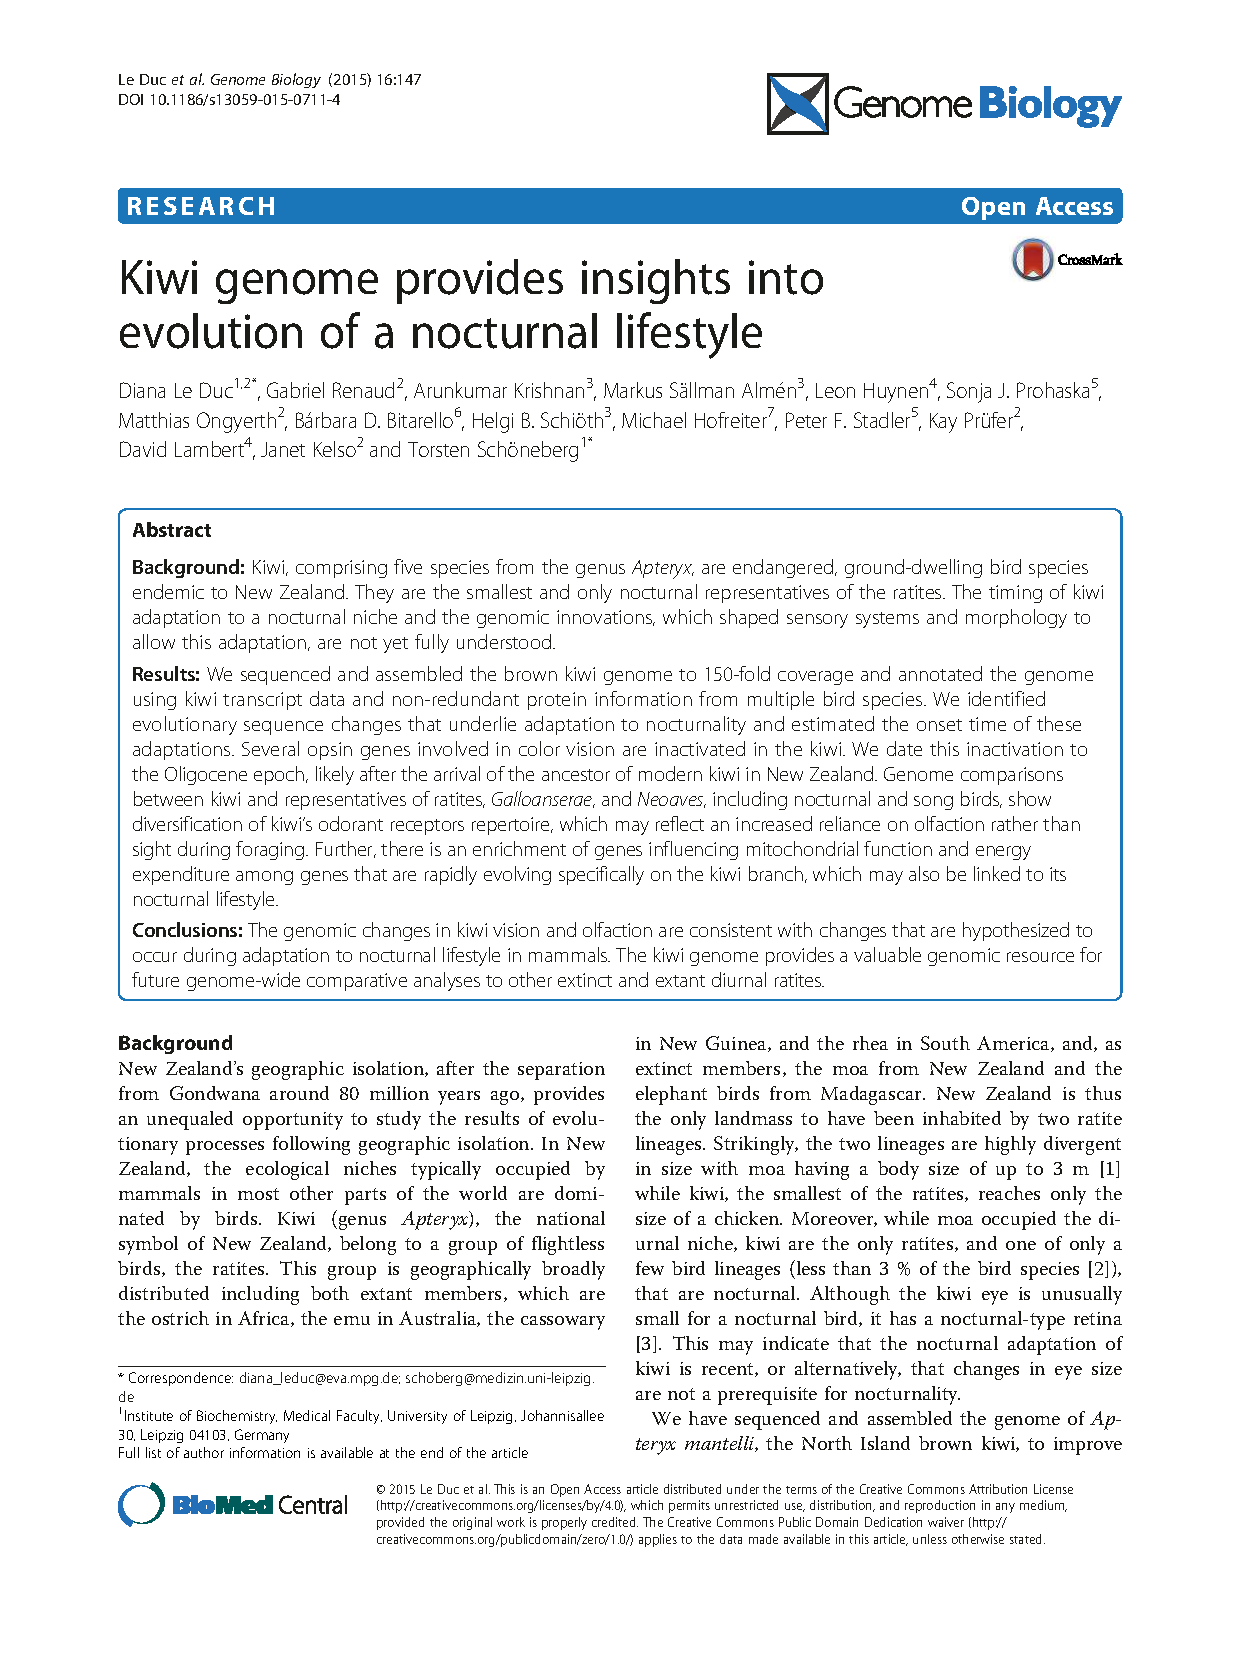
\includepdf[
            pages=-,
            width=189mm,
            height=250mm,
            offset=15pt 0pt,
            pagecommand={\pagestyle{plain}}
            ]{Appendix/small_kiwi.pdf}


 %%%%%%%%%%%%%%%%%%%%%%%%%%%%%%%%
 %%%%%%%%%%%%%%%%%%%%%%%%%%%%%%%%
 %%%%%%%%%%%%%%%%%%%%%%%%%%%%%%%%
 %%%%%%%%%%%%%%%%%%%%%%%%%%%%%%%%
 
\section{Apêndice A.4.}


Cópia pessoal do manuscrito \enquote{Heterogeneity of dN/dS Ratios at the Classical HLA Class I Genes over Divergence Time and Across the Allelic Phylogeny}: \emph{Journal of Molecular Evolution} (2015) 82(1): 38-50. O artigo em sua versão final (pós-processamento editorial) não está liberado para ser re-distribuído a partir deste documento, uma vez que o mesmo não é \enquote{Open Access}. Portanto, disponibilizo a versão aceita para publicação, porém sem a formatação da revista -- esta encontra-se disponível pelo DOI \href{http://link.springer.com/article/10.1007/s00239-015-9713-9}{10.1007/s00239-015-9713-9}.
 
Esse artigo é o resultado do meu trabalho de mestrado, que foi aprimorado ao longo do meu doutorado. Ele tem elementos em comum com o artigo apresentado no apêndice A.2, pois em ambos investigamos as unidades de seleção nos genes HLA: aqui, linhagens alélicas; no outro artigo (A.2), supertipos. 

Neste trabalho, fui orientada por Diogo Meyer, que concebeu as ideias originais do projeto. Ambos desenvolvemos as metodologias a serem adotadas ao longo do projeto. Executei todas as análises e redigi o manuscrito juntamente com DM. RSF e eu fizemos a detecção de sequências recombinantes e todos os co-autores participaram na discussão e verificação dos resultados.


 %A Springer diz no Transfer of Copyright deles que eu posso usar essa versão em dissertações.
 %"The author retains the right to use his/her article for his/her further scientific career by including the final published journal article in other publications such as dissertations and postdoctoral qualifications pro- vided acknowledgement is given to the original source of publication."
 
 %mas eu fico com medo porque essa tese vai ser disponibilizada online e isso apareceria nas buscas pelo nome desse artigo, de forma que alguém que baixasse a tese poderia ler o artigo. Antes de submeter a tese seria bom ter certeza (mandar um email pra Springer).


%%%%%%%%%%%%%%%%%%%%%%%%%%%%%%%%
%%%%%%%%%%%%%%%%%%%%%%%%%%%%%%%%
%%%%%%%%%%%%%%%%%%%%%%%%%%%%%%%%
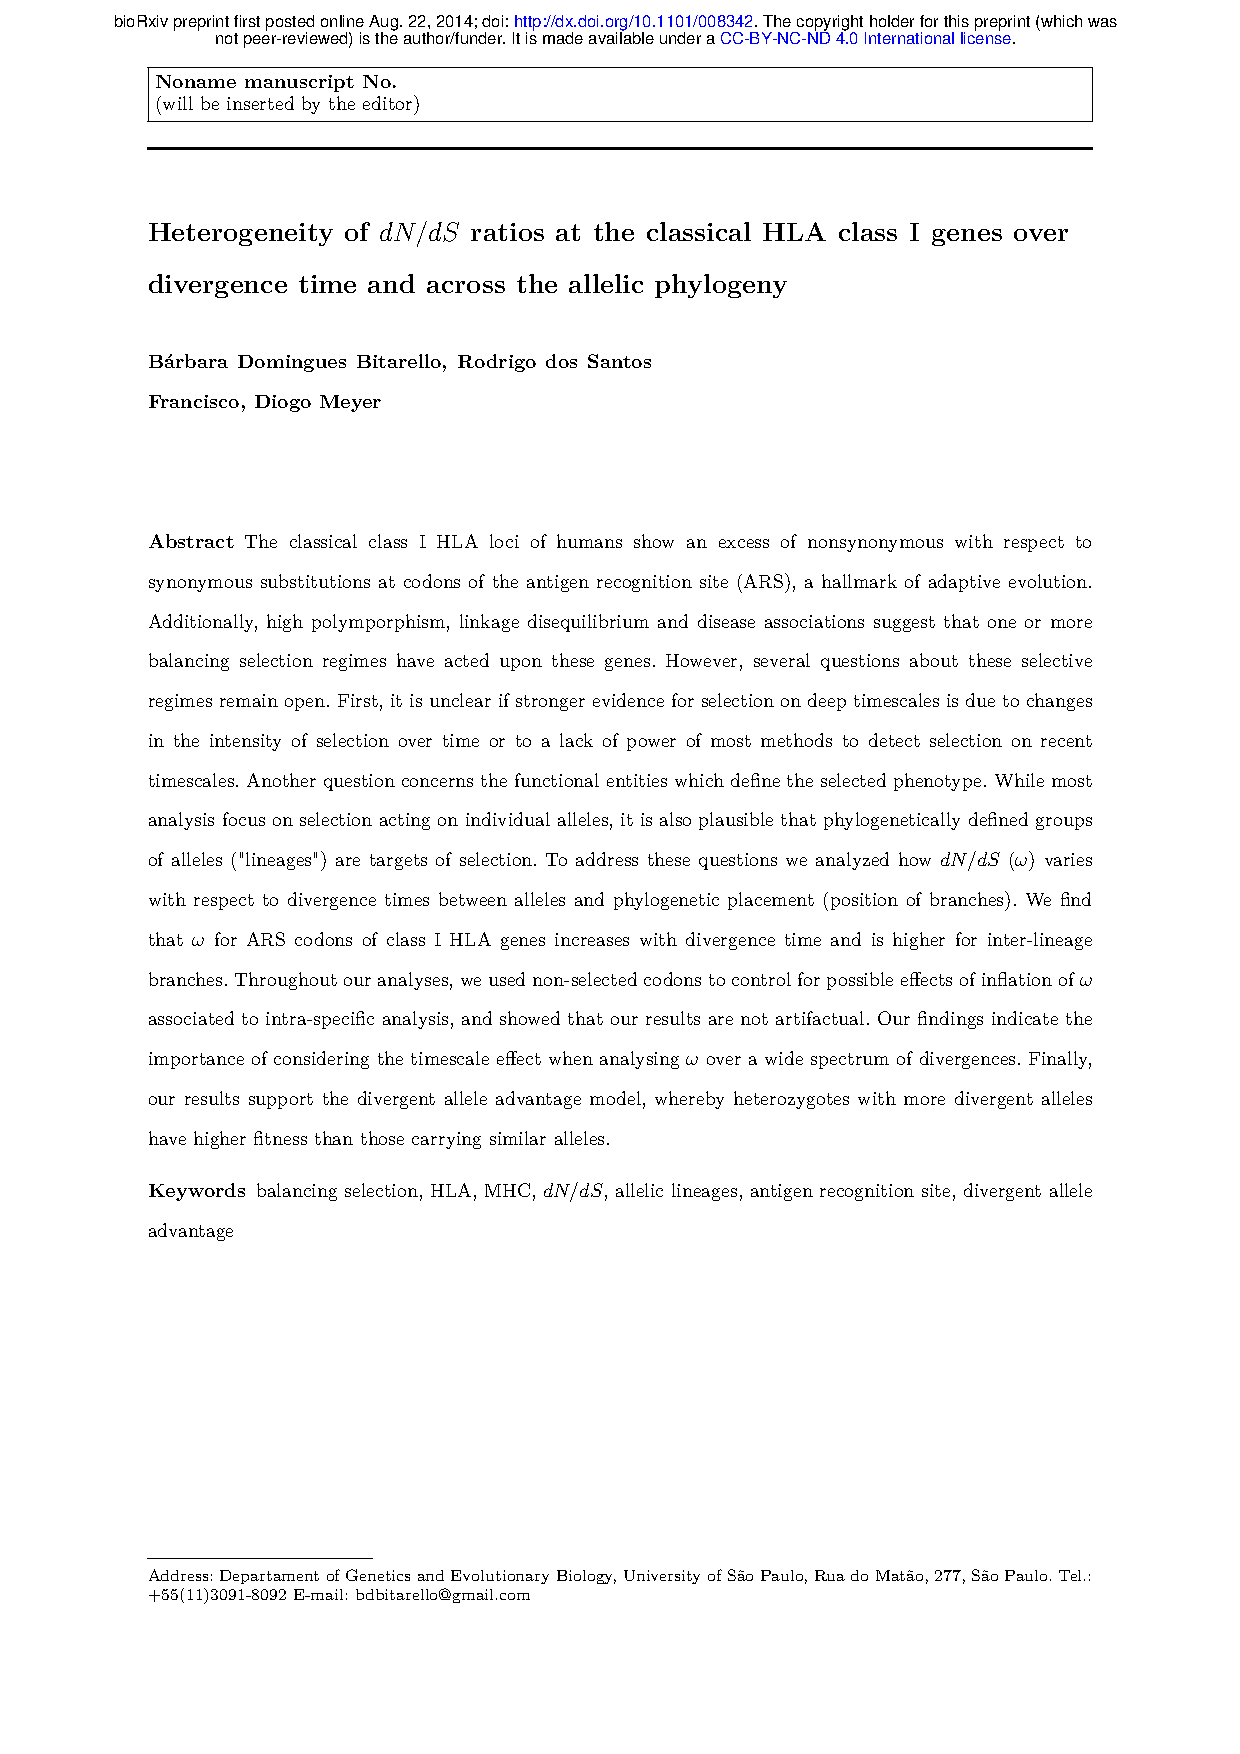
\includepdf[
            pages=-,
            width=189mm,
            height=255mm,
            offset=15pt 0pt,
            pagecommand={\pagestyle{plain}}
            ]{Appendix/small_dNdS.pdf}
            

